%!TEX root = ../thesis.tex
\chapter{Background}
\label{chap:background}

Studying ways to bridge the gap between the fields of MAS and MABS has been the subject of several works and resulted in the development of different tools, each with its own purpose. Some works were in search of increased performance for MABS; others tried to cater specific needs such as providing an appropriate learning environment. This chapter describes some works that are relevant to this thesis and makes a comparison between some of them.

\section{Related Work}
% Study of similar frameworks for agent based simulation
Several frameworks exist that offer support to the development of MAS or MABS. Some are domain specific, meaning that their purpose was well defined in their conception. MASeRaTi\cite{ahlbrecht2014scalable}, MATSim\cite{balmer2008agent} and SUMO\cite{SUMO2012} are some examples of MABS frameworks for traffic and transports simulation. 

Other works like Repast\cite{collier2003repast}, NetLogo\cite{tisue2004netlogo}, GALATEA\cite{davila2000galatea} and Plasma \cite{warden2010towards} are considered general-purpose. This list comprises only tools that are free and open source and is not meant to be exhaustive. 

Some works propose approaches that are very similar to the solution proposed in this thesis, namely the bridging of the domains of MAS and Simulation. MISIA, JRep and Plasma were built on top of JADE to create a simulation environment based on it. These three works were studied with more detailed due to these similarities.

\subsection{MISIA}
MISIA is a middleware whose goal is to enhance the simulation of intelligent agents and to allow the visualization and analysis of agent's behaviour. It was developed by the Bioinformatic, Intelligent Systems and Educational Technology Research Group (BISITE) from Universidad de Salamanca\footnote{http://bisite.usal.es/}. It is no longer an active project; as a research experiment, work on this middleware evolved into other more specific tools.

MISIA's approach, as suggested by Figure \ref{fig:misia}, is to use a middle layer that acts as the bridge between two other layers that interact with JADE and Repast. By extending the agents in Repast and JADE, communicating through a coordinator and synchronizing their state, these agents work as a single one.

\begin{figure}[h]
	\centering
	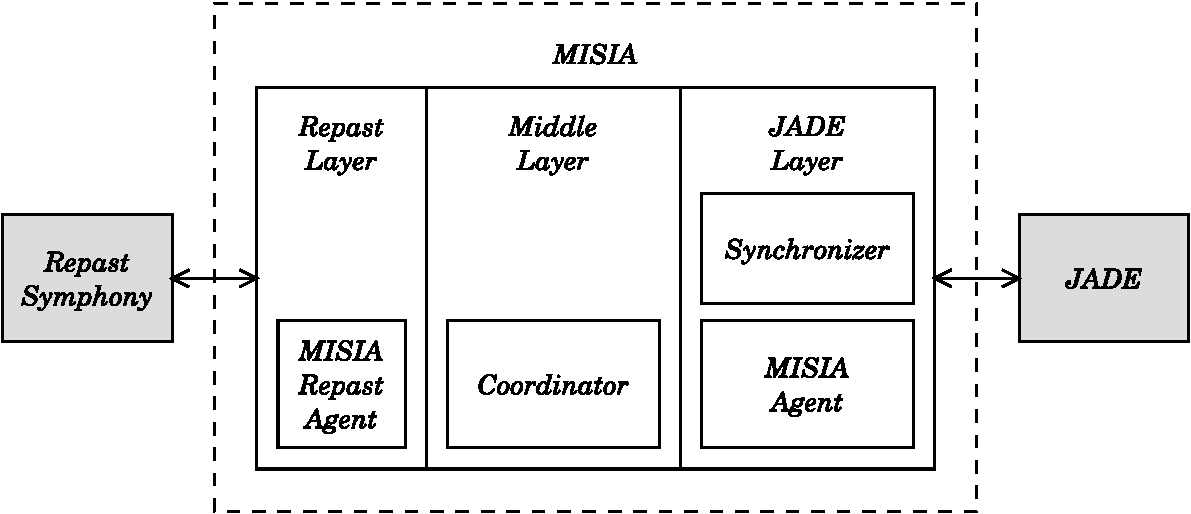
\includegraphics[width=0.75\linewidth]{figures/MISIA.pdf}
	\caption[MISIA's architecture]{High-level representation of MISIA's architecture (adapted from \cite{garcia2011misia})}
	\label{fig:misia}
\end{figure}

One of the challenges identified by the authors when re-implementing the FIPA interaction protocols was synchronizing them with the Repast tick-based simulation model. Given JADE's event-driven architecture, MISIA proposes the use of a coordinator agent that informs the JADE-Agent when a tick has passed. It also proposes its own implementation of the interaction protocols supported by JADE, making them tick-friendly.

\subsection{JRep}
JRep is another platform for integrating JADE and Repast Symphony in the same framework, by means of a middleware. To demonstrate its use, the authors present an example of a smart airport and how it can be simulated using JREP.

JRep's approach is not as complex as MISIA's.
By having the Repast Simphony agent encapsulate a JADE agent representation, synchronization is immediate and is assured without requiring an external coordinator.
The two agent representations take care of synchronizing any state changes.
Figure \ref{fig:jrep} represents the basic structure of JRep.

\begin{figure}[h]
	\centering
	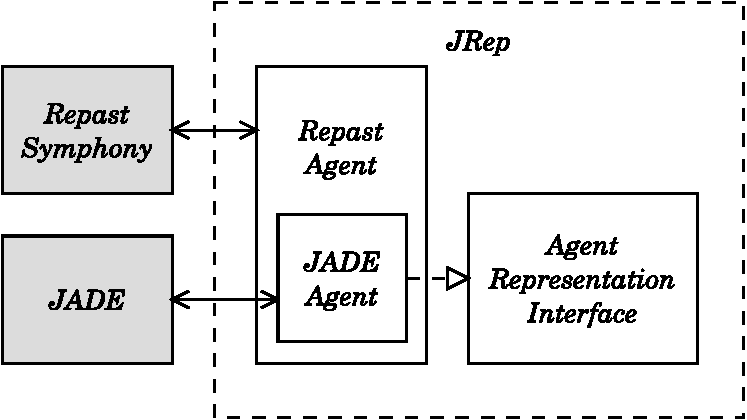
\includegraphics[width=0.5\linewidth]{figures/jrep.pdf}
	\caption[JRep's architecture]{High-level representation of JRep's architecture (adapted from \cite{gormer2011jrep})}
	\label{fig:jrep}
\end{figure}

Each agent takes care of interfacing their respective frameworks. The interaction between agents in JRep is performed using FIPA ACL and the protocol implementations are those provided by the JADE platform. Similarly to MISIA, an Agent Representation Interface is used to introduce the concept of schedule in the JADE agent.

\subsection{PlaSMA}
Unlike the two previous frameworks, the PlaSMA system is based solely on the JADE platform. The distributed simulation is synchronized by entities called ``Controllers'' who communicate with the ``Top Controller'', keeping the pace of the simulation and handling agent lifecycle management as well. Figure \ref{fig:plasma} illustrates this architecture. PlaSMA, unlike MISIA and JRep, is still an active project.

\begin{figure}[h]
	\centering
	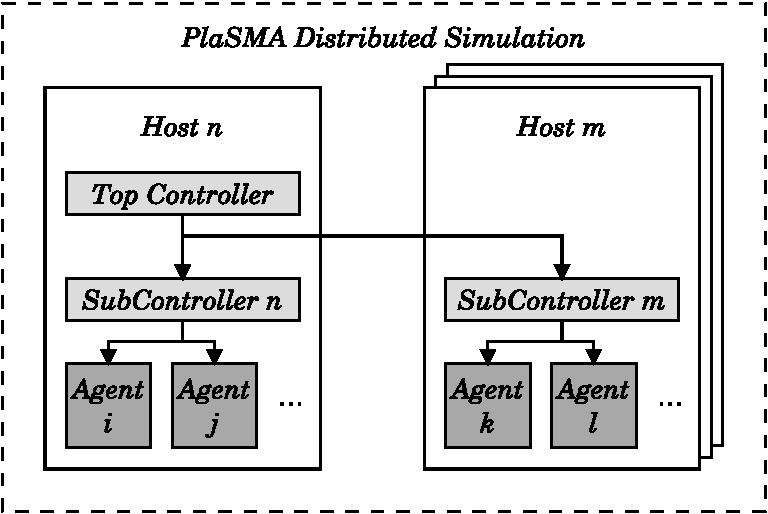
\includegraphics[width=0.5\linewidth]{figures/PlaSMA.pdf}
	\caption[PlaSMA's architecture]{High-level representation of PlaSMA's architecture (adapted from \cite{warden2010towards})}
	\label{fig:plasma}
\end{figure}

JADE is a very rich platform but, for many simulation scenarios, the overhead introduced by it has a significant impact on simulation performance \cite{mengistu2008scalability}.

Even though both MISIA and JRep attempt to integrate the features from both JADE and Repast, as far as Repast simulations are concerned JADE's multi-threaded infrastructure affects their performance very significantly. The main advantage of our approach is, therefore, the possibility of using Repast with JADE features, namely FIPA specifications including interaction protocols, without the need to interface with JADE. 

\section{JADE and Repast}
\label{sec:jade-repast}

To achieve the goals of this thesis, two frameworks were chosen: JADE and Repast. Both are very popular and in widespread use and have been the foundation of the creation of other tools. They are also free and open source and extensively documented.

JADE is a framework for development of FIPA-compliant fully featured MAS. It aims at simplifying the creation of distributed agent applications by seamlessly hiding all complexity regarding its distributed architecture, including the tasks of agent discovery and the handling of messages.

Repast is a toolkit that provides an environment for the creation of MABS using POJO\footnote{Plain Old Java Objects}. It makes it fairly simple to collect agent data and generate displays for it, including charts, grids and others.


\begin{table}[h]
	\caption{Summary of JADE and Repast features.}
	\label{tab:jadevsrep}
	\begin{center}
		\begin{tabular}{l|cc}
		\hline

		\hline
		\textbf{} & \textbf{JADE} & \textbf{Repast} \\ %& \textbf{Cougaar} \\
		\hline
			Communication & FIPA ACL &  Method calls  \\ %& Serialized Object \\
						  &			 &  Shared resources \\
		\hline
			Distribution & Yes & No \\ %& Yes \\
		\hline
			Simulation Tools & No & Yes \\ %& Yes \\
		\hline
			Scalability & Limited & High \\ %& High \\
		\hline
			Ontologies & Yes & No \\ %& Yes\\
		\hline
			Open Source & Yes & Yes \\ %& Yes\\
		\hline
			Agent Execution & Behaviour-based & Schedule-based  \\ %&  \\
							& Multi-threaded & Single-threaded \\ %&  \\
							& Event-driven   & Tick-driven 	   \\ %&  \\
							& Assync		 & Sync 		   \\ %&  \\
		\hline
		\end{tabular}
	\end{center}
\end{table}

In JADE, as table \ref{tab:jadevsrep} illustrates, agents execute in separate threads and while this architecture facilitates the platform's distribution, JADE's agent are heavy in terms of resources. Experiments with JADE show that the platform's scalability is limited in number of agents and that the global system performance drops quickly for large number of agents \cite{mengistu2008scalability} \cite{garcia2011misia}. This further strengthens the idea that using JADE or a JADE-Repast hybrid, as describe in the related work, is not the best course of action is performance is an important issue.

In Repast, agent execution is scheduled manually. An agent class can contain annotations that indicate which methods should be called and when (for instance every tick or every 100 ticks). This approach is very flexible, allowing to schedule any method but more complex structures are non-existent in Repast.

In contrast, JADE agent actions can be executed in their setup and takedown, but most are encapsulated in objects called Behaviours. JADE has many different kinds of behaviours that function in different ways, such as running one single task once or running them cyclically. Other behaviours implement FIPA interaction protocols, which agents can use to interact with other agents.

Agents, as well as their behaviours, go through different states, as Figure \ref{fig:jade_fluxogram} suggests. As each agent in JADE runs in a thread, each one is dedicated solely to the agent's behaviours. These behaviours are executed consecutively until the agents is taken down and each behaviour stops being scheduled when it is ``done'' -- indicated by the return value of the method \texttt{done()}.

\begin{figure}[h]
	\centering
	\includegraphics[width=0.7\linewidth]{figures/jade_fluxogram.pdf}
	\caption[JADE Behaviour execution states]{JADE Behaviour execution states and events (adapted from \cite{bellifemine2007developing})}
	\label{fig:jade_fluxogram}
\end{figure}

%!TEX root = ../thesis.tex
\section{FIPA Specifications in JADE} % (fold)
\label{sec:fipa}

% Intro to FIPA in JADE/API
\apiname{} closely follows JADE's architecture regarding the use of protocols and services specified by FIPA. 
%The architecture of the API described in this paper includes multiple concepts proposed by FIPA: the \gls{DF}, the \gls{MTS}, the \gls{AMS}, the \gls{ACL} Message and the Interaction Protocols. The following is a brief description of these concepts and of how JADE uses and implements them.

%\begin{figure}
%	\centering
%	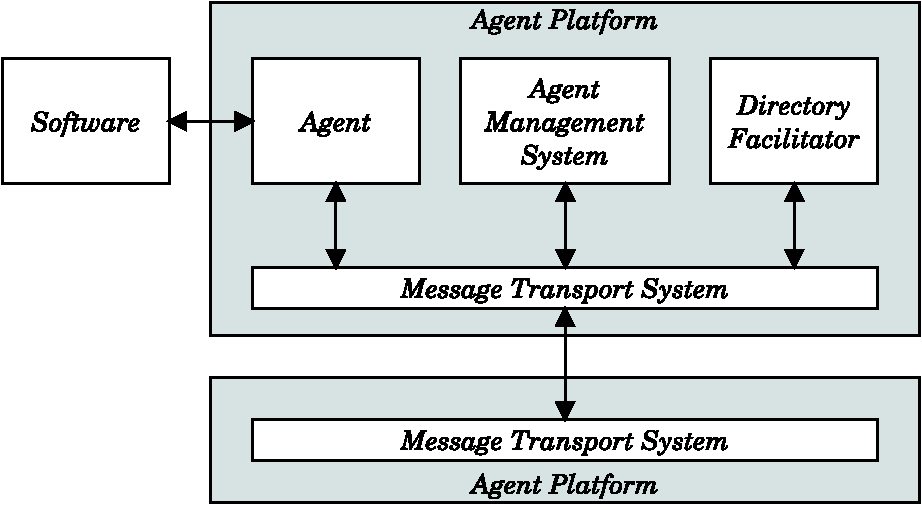
\includegraphics[width=2.5in]{figures/pdf/AMSdiagram.pdf}
%	\caption{
%		Agent Management Reference Model, as specified by FIPA and implemented by JADE. \apiname{} only supports a single Agent Platform.
%	}
%	\label{fig:AMSdiagram}
%\end{figure}

% DF 
The Directory Service (DF) is a component that provides a yellow page service and is part of the FIPA Agent Management Specification. It allows one agent to perform searches about agents rendering specific services. Only agents that are registered in the DF will be indexed and agents can register and deregister themselves at any time.

% DF Agent Description
When searching the DF, agents can use templates that filter the search results. A DF Agent Description represents this template and contains the fields listed in Table \ref{tab:dfAgentDescription}.sim


% MTS
The MTS is a service for transportation of ACL messages between agents. It is responsible for resolving agent addresses, in order to be able to deliver those messages. The MTS may request information from the AMS to perform this address resolution.

% AMS
The AMS is a mandatory component in FIPA-compliant agent platforms. Its purpose is to manage the agent platform, namely the creating and deletion of agents.

% ACL Message
The ACL Message is the envelope that contains the details for communication. The Agent Comunication Language (ACL) stipulates what fields a message should contain. Table \ref{tab:fipaACLMessage} was adapted from the FIPA ACL Message structure specification and contains the list of fields in a message. Not all of them are mandatory. FIPA specifies the \texttt{performative} as the only mandatory field, although the \texttt{sender}, \texttt{receiver} and \texttt{content} are expected to be present.

\begin{table}
	\normalsize
	\caption{FIPA ACL Message Parameters}
	\label{tab:fipaACLMessage}
	\begin{center}
		\fboxsep1pt
		\begin{tabular}{c|c}
		\hline
		\textbf{Parameter} & \textbf{Category of Parameters} \\
		\hline
		\colorbox{Apricot}{\texttt{performative}} & Type of communicative acts \\
		\hline
		\colorbox{Apricot}{\texttt{sender}} & \multirow{3}{*}{Participant in communication} \\
		\cline{1-1}
		\colorbox{Apricot}{\texttt{receiver}} \\
		\cline{1-1}
		\texttt{reply-to}  \\
		\hline
		\colorbox{Apricot}{\texttt{content}} & Content of message \\
		\hline
		\texttt{language} & \multirow{3}{*}{Description of Content} \\
		\cline{1-1}
		\texttt{encoding} \\
		\cline{1-1}
		\colorbox{Apricot}{\texttt{ontology}} \\
		\hline
		\colorbox{Apricot}{\texttt{protocol}} & \multirow{5}{*}{Control of conversation} \\
		\cline{1-1}
		\colorbox{Apricot}{\texttt{conversation-id}} \\
		\cline{1-1}
		\texttt{reply-with} \\
		\cline{1-1}
		\texttt{in-reply-to} \\
		\cline{1-1}
		\colorbox{Apricot}{\texttt{reply-by}} \\
		\hline
		\end{tabular}
	\end{center}
\end{table} 

% Protocols In FIPA
FIPA Interaction Protocols typify communication interactions among agents by specifying two roles: initiator (the agent starting the interaction) and responder (a participant in the interaction). Each protocol defines precisely which messages are sent by each role ad in which sequence.

% Behaviors in JADE
In JADE, every agent activity is programmed through the notion o behaviours. For interaction protocols, typically behaviour-pairs are used for each side of the interaction, and JADE's API supports the most important protocols with built-in initiator and responder behaviours.
% Implementing these protocols.
In order to create an application using these protocols, programmers only need to extend these behaviours and implement the message handlers.
All the complexity regarding the interaction and networking infrastructure is hidden and taken care of by JADE, allowing the programmer to focus on the implementation of agent behaviour.

\subsection{FIPA Interaction Protocols}

To provide a more solid background to the protocols mentioned in this thesis, it's relevant to perform a deeper analysys of them. The two protocols currently supported in the API, as will be explained further ahead in Chapter \ref{chap:solution}, are the FIPA Request, FIPA Query and the FIPA Contract Net. JADE supports a few other protocols, namely FIPA Propose, Iterated FIPA Request and Query and FIPA Subscribe.

\begin{table}
	\normalsize
	\caption{Interaction protocols supported in JADE}
	\label{tab:fipa_protos}
	\begin{center}
		\fboxsep1pt
		\begin{tabular}{c|c|c}
		\hline
		\textbf{Protocol(s)} & \textbf{Initiator class} & \textbf{Initiator class} \\
		\hline
		FIPA request 	& \multirow{2}{*}{AchieveREInitiator} & \multirow{2}{*}{AchieveREResponder}\\
		FIPA Query 		& \\
		\hline
		\multirow{2}{*}{FIPA Contract Net} & \multirow{2}{*}{ContractNetInitiator} & ContractNetResponder \\
		 &  & SSContractNetResponder \\
		\hline
		\end{tabular}
	\end{center}
\end{table}


In JADE, the AchieveRE protocol encompases the multiple ``request-like'' behaviours such as FIPA-Request. It is a simple protocol with three moments of interaction, as Figure \ref{fig:FIPA_request_proto} shows: a request, a response of acceptance or refusal and a facultative result notification. JADE allows the use of other interaction protocols with the AchieveRE: FIPA-query, FIPA-Request-When, FIPA-recruiting and FIPA-brokering. Interaction using this protocol can be 1:1 or 1:N.

The Contract Net protocol starts with a Call for Proposals (CFP) sent to one or more agents, which can reply with a proposal or with a refusal to propose. The initiator can then accept or reject the proposals. As in FIPA-Request, the final result notification is facultative. The ContractNetResponder class from JADE resets itself after terminating the protocol and stays waiting for new CFPs. JADE provides an alternative responder class called SSContractNetResponder that terminates after a single session (SS stands for single session).

\begin{figure}[ht]
	\centering
    \begin{subfigure}[b]{0.44\textwidth}
		\centering
		\includegraphics[height=4in]{figures/FIPA_request_proto.pdf}
		\caption[FIPA-Request protocol]{FIPA-Request protocol}
		\label{fig:FIPA_request_proto}
    \end{subfigure}%
    \begin{subfigure}[b]{0.54\textwidth}
		\centering
		\includegraphics[height=4in]{figures/FIPA_contnet_proto.pdf}
		\caption[FIPA-Contract-Net protocol]{FIPA-Contract-Net protocol}
		\label{fig:FIPA_contnet_proto}
    \end{subfigure}
    \caption[]{Sequence diagrams for the protocols Contract Net and Request. \\Figures are from the FIPA specifications website \footnote{http://fipa.org/})}
    \label{fig:FIPA_Protocols}
\end{figure}


\section{Summary}
Although the specific problem of reimplementing JADE features in Repast using a pure Java approach has not been approached before in the available literature, it is clear that some related work is useful in the definition of the solution proposed in this thesis. 

JREP and MISIA show that interoperability between the two frameworks is possible and they helped understand the limitations of each framework. They both attempted to complement Repast's lack of communication protocols by creating an interface with JADE's implementation of FIPA interaction protocols. The usefulness of these works is limited, though, since the source code is not readily available and neither project is still being developed and supported.

Other works related to the integration of features from Repast and JADE are available and these were selected as the most relevant. While the goal of this thesis is not to use both frameworks simultaneously, these works give a valuable insight into the shortcomings of both frameworks as well as providing some interesting comparisons between their features. Open source projects exist that contemplate the use of FIPA ACL as a library, but none was found to be actively maintained or properly documented. Therefore, this thesis contemplates the creation of a Java API that brings JADE-like features to simulation tools, including FIPA standards.